\documentclass[onecolumn, draftclsnofoot,10pt, compsoc]{IEEEtran}
\usepackage{graphicx}
\usepackage{url}
\usepackage{setspace}
\usepackage{float}

\usepackage{geometry}
\geometry{textheight=9.5in, textwidth=7in}

% 1. Fill in these details
\def \CapstoneTeamName{			Velocity-Raptors}
\def \CapstoneTeamNumber{		37}
\def \GroupMemberOne{			Alex Bailey}
\def \GroupMemberTwo{			Dylan Washburne}
\def \GroupMemberThree{			Benjamin Wick}
\def \CapstoneProjectName{		Object Velocity Tracking}
\def \CapstoneSponsorCompany{}
\def \CapstoneSponsorPerson{		Alex Neighbors}

% 2. Uncomment the appropriate line below so that the document type works
\def \DocType{		%Problem Statement
				%Requirements Document
				%Technology Review
				Design Document
				%Winter Progress Report
				}
			
\newcommand{\NameSigPair}[1]{\par
\makebox[2.75in][r]{#1} \hfil 	\makebox[3.25in]{\makebox[2.25in]{\hrulefill} \hfill		\makebox[.75in]{\hrulefill}}
\par\vspace{-12pt} \textit{\tiny\noindent
\makebox[2.75in]{} \hfil		\makebox[3.25in]{\makebox[2.25in][r]{Signature} \hfill	\makebox[.75in][r]{Date}}}}
% 3. If the document is not to be signed, uncomment the RENEWcommand below
%\renewcommand{\NameSigPair}[1]{#1}

%%%%%%%%%%%%%%%%%%%%%%%%%%%%%%%%%%%%%%%
\begin{document}
\begin{titlepage}
    \pagenumbering{gobble}
    \begin{singlespace}
    	
\includegraphics[height=4cm]{coe_v_spot1}
        \hfill 
        % 4. If you have a logo, use this includegraphics command to put it on the coversheet.
        %\includegraphics[height=4cm]{CompanyLogo}   
        \par\vspace{.2in}
        \centering
        \scshape{
            \huge CS Capstone \DocType \par
            {\large\today}\par
            \vspace{.5in}
            \textbf{\Huge\CapstoneProjectName}\par
            \vfill
            {\large Prepared for}\par
            \Huge \CapstoneSponsorCompany\par
            \vspace{5pt}
            {\Large\NameSigPair{\CapstoneSponsorPerson}\par}
            {\large Prepared by }\par
            Group\CapstoneTeamNumber\par
            % 5. comment out the line below this one if you do not wish to name your team
            %\CapstoneTeamName\par 
            \vspace{5pt}
            {\Large
                \NameSigPair{\GroupMemberOne}\par
                \NameSigPair{\GroupMemberTwo}\par
                \NameSigPair{\GroupMemberThree}\par
            }
            \vspace{20pt}
        }
        \begin{abstract}
        % 6. Fill in your abstract    
        	The Object Speed Tracking system incorporates many different technologies to make it possible.
This includes computer vision libraries, object tracking methods, speed algorithms, and the user interface.
This document shows the intended design for the system and how it will incorporate the technology need to meet the system requirements.
            
        \end{abstract}     
    \end{singlespace}
\end{titlepage}
\newpage
\pagenumbering{arabic}
\tableofcontents
% 7. uncomment this (if applicable). Consider adding a page break.
%\listoffigures
%\listoftables
\clearpage

% 8. now you write!
\section{Introduction}
\subsection{Purpose}
The purpose of this document is to give the necessary and required information to effectively define our systems design and give our team guidance to execute the system throughout the implementation process.

\subsection{Scope}
This system intends to utilize a live video feed in order to determine the speed of an object.
The software will be able to identify a specific type of object, such as a person, or RC car and then calculate the object's speed and display it to the user on a windows application.
This offers an alternative method to track speeds of moving objects.

%\subsection{Intended Audience}
%This document is intended for the use of the developers, who will implement the system, as well as the stakeholders and clients involved.

\subsection{Context}
The Object Speed Tracking system will be a windows application that utilizes a Microsoft Xbox 360 Kinect camera along with a computer vision library to track and calculate the speed of moving objects.
This project is intended for a class at Oregon State University. Our goal is to implement the project design.
Future development plans will be based on feature needs and success of project determined by the client.

%\subsection{References}

\subsection{Glossary}
\begin{center}
	\begin{tabular}{|p{4cm}|p{12cm}|}
    
		\hline
		\textbf{Term} & \textbf{Definition} \\
		\hline
		API (Application Program Interface) & A particular set of rules and specifications that software programs can follow to communicate with each other. \\
		\hline
		Computer vision & The ability for the computer to extract, analyze and understand from an image or video. \\
		\hline
		Object & The entity being tracked by the video feed.  \\
		\hline
		Kinect camera & A type of camera that has in infrared camera and color camera as well as a infrared light projector.  \\
		\hline
    	User Interface (UI) & The visual part of the application in which the user will interact with.  \\
		\hline
	
	\end{tabular}
\end{center}

\section{Body}
\subsection{Identified Stakeholders}
The main stakeholder for our product is Alex Neighbors, as the client of our project.
Alex Neighbors' concerns for our product is to create a product that is able to track objects and calculate the speed. This project is a proof of concept for which in the future, more different systems can be used and our project can be enhanced to fit the needs of others.

There are many different applications and users that can use our system who would be identified as stakeholders.
We will now discuss possible object types, the stakeholders depending on the type and their concerns.
Law enforcement would be a possible stakeholder for this technology as it could be used in place of current speed limit enforcement technology.
Their concerns could be how many vehicles it can track at a time or the accuracy of the velocity.

Sports teams and sports analysts could be stakeholders for analyzing how the players are moving.
Anyone group trying to study the movement of groups of people, such as someone trying to see how fast people are able to evacuate in an emergency, could be a stakeholder.
Their concerns could be the speed of the calculation or speed and consistent of the frame-rate.


\subsection{Interaction Viewpoint}
\subsubsection{Viewpoint Description}

The Interaction Viewpoint describes how the different pieces of our product work together and what is sent back and forth between them. 

\begin{figure}[H]
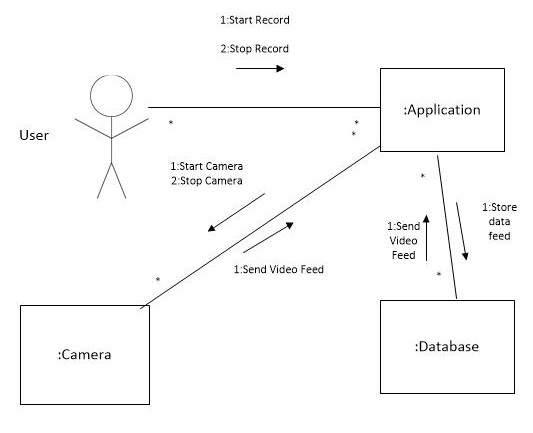
\includegraphics[scale=.7]{interaction_diagram}
\caption{UML Communication Diagram}
\label{inter}
\end{figure}


\subsubsection{Design Concerns}

The concerns for this Viewpoint are how the different components of our product will be interacting, which components will be interacting with each other, and what information will be passed between each component.

\subsubsection{Design Elements}

There are four elements in this viewpoint.
The first is the user of the product.
To keep the user interface simple the user will be able to start the recording and stop the recording.
The second element is the application.
This will be run on a computer of the user choice.
The application will handle the interactions with the camera and database.
It will send the start and stop signals to the camera and send the video for storage to the database.
The application will also be able to receive a video stream from the database in order to recalculate the data.
The third element is the camera.
This will most likely be connected to the computer running the application, but not necessarily. The camera will record video when signaled and send the video feed to the application.
The fourth element is the database.
This will most likely be run on the same computer running the application, but not necessarily.
This element will receive the video for storage from the application and will also send a video to the application for recalculating the data.

\subsection{Information Viewpoint}
\subsubsection{Viewpoint Description}
The purpose of the Information viewpoint is to describe how the data will be stored for the video radar software. The goal is to maximize efficiency and accuracy. There are two main entities within this viewpoint which include video storage and results storage.

\subsubsection{Design Concerns} 
Concerns with information include storing the correct data, data management strategies and data access schemes.

\begin{figure}[H]
\includegraphics[scale=.7]{data}
\caption{Flowchart diagram for information storage.}
\label{fig:data}
\end{figure}

\subsubsection{Design Elements}
The user will interact directly with the application.
Once setting up the system, the Kinect camera will identify the distance to objects and then the application will calculate the speed at which it is moving.
This information is displayed to the user on the screen as well as stored in a separate text file.
The first element is the video storage.
The live video feed will have be captured and stored.
To do so we will implement a video capture class that is provided in the OpenCV library.
This class will capture the live video feed and store the video in MP4 format into a file.
The second element includes the final results being stored.
The final results will be stored into a text file.
The data that will be stored includes the object number for reference with the video, the speed of the object, and the time the object's speed was calculated.
This will be implemented with a class called "storeResults".
This class will extract the data needed from the calculation classes and the video feed and write it into a separate text file.

\subsection{Context Viewpoint}
\subsubsection{Viewpoint Description}
The Context Viewpoint describes the specific details of our project which are vital to its overall success, while sometimes not applying to any singular other category.

\begin{figure}[H]
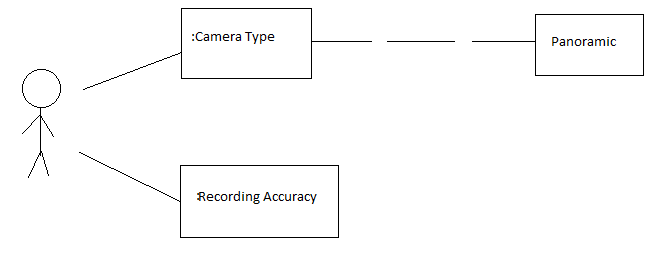
\includegraphics[scale=.8]{context-uml}
\caption{UML Use Case Diagram of the project's context.}
\label{fig:context}
\end{figure}

\subsubsection{Design Concerns}
This Viewpoint is concerned with the specific issues which affect the performance of many other aspects of the project, which are to be adhered to throughout the building and testing of the project.

\subsubsection{Design Elements}
The first element is that the finished project will be able to return the velocity of specified objects in frame.
The returned velocities will be within 90\% of their actual velocities.
The upcoming elements discussed are general pointers on how to achieve that outcome.
The second element is that the project will utilize a Kinect camera to receive the video data.
The Kinect will generate information about the depth of objects in the frame.
Our client provided us with the Kinect, due to its nature to more synchronize shutter timing and create depth information.
The next element is that the cameras must have enough range to accurately determine an object's depth.
We believe that the Kinect's 6 meter range will be sufficient for our tracking purposes.


\subsection{Algorithm Viewpoint}
\subsubsection{Viewpoint Description}
This viewpoint describes method used for calculating the velocity of the desired object.

\subsubsection{Design Concerns}
The concerns of this viewpoint are determining the logic for calculating the velocity of the desired object type, determining where data would be coming from and sent to, and when data should be stored for later use and when it should be retrieved.

\begin{figure}[H]
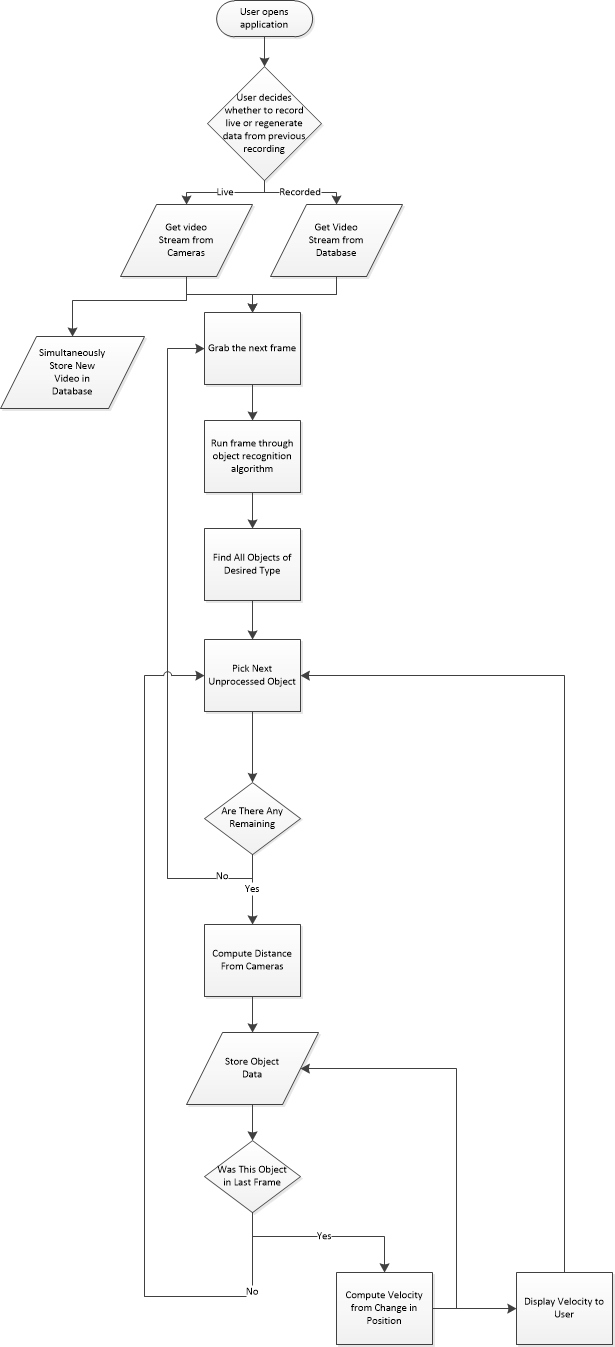
\includegraphics[scale=.68]{flowchart}
\caption{Flowchart Diagram of Calculating Object Velocity}
\label{fig:flowchart}
\end{figure}


\subsubsection{Design Elements}
The data elements represent the database. 
The element that displays velocity to user will print the information to the application window, with a way of showing the user which object is being referenced by that velocity.


\subsubsection{Processing Attribute}
The prerequisites for this flowchart is for the application to have been activated, the cameras be plugged in, the database connected to the application. 
The loop for finding the next object to be processed withing the frame will continue up to the minimum number of objects our product must recognize, but may or may not process the remaining objects depending on the limitation of the system.
The priority of the algorithm will be to compute the velocities of the minimum number of vehicles, followed by frame-rate for displaying to velocity to the user.



%\subsection{Resources Viewpoint}

\subsection{Design Rationale}
The main rational behind the creation of our product and this document was the concerns supplied by our client Alex Neighbors, making a proof of concept for a product that can replace the current technology for object velocity tracking by making up for the pitfalls of the current technology.
So we designed our product around how we could make up for the pitfalls, such as how a camera would have the ability to see and therefore track several object whereas one of the current methods, a radar gun, could not.
The choice of our camera depended largely on price, convenience, and the ability to track objects.
We decided the Kinect would be a good choice because of the 3D sensors it uses to determine depth.
The Kinect also was created to track people which gave it an edge on other camera choices.

\end{document}